\documentclass{article}
%调用名为 article 的文档类
\usepackage[utf8]{inputenc}
\usepackage{graphicx}

\title{TAS Scheduling for Real-Time Forwarding of Emergency Event Traffic in TSN}
\author{zhangguangyu082 }
\date{December 2021}

\begin{document}
%只有在 document 环境中的内容,才会被正常输出到文档中
\maketitle
%控制序列 maketitle:能将在导言区中定义的标题、作者、日期按照预定的格式展现出来
\section{Introduction}
Industrial systems that utilize advanced network technologies have been developed in various fields such as audiovideo, smart factories, and automotive networks, to provide differentiated quality of service (QoS) to different applications and services.
\cite{ref1}

\begin{figure}[h!]
\centering
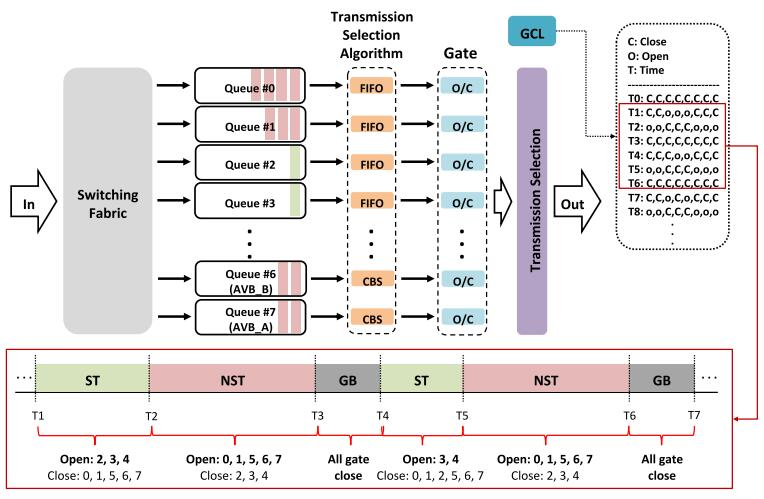
\includegraphics[scale=0.4]{TAS1}
\caption{IEEE 802.1Qbv Time Aware Shaping}
\label{fig:label}
\end{figure}

\section{Conclusion}
In this paper, we have shown that unscheduled high-priority emergency event traffic may induce significant delay and jitter to scheduled traffic in IEEE 802.1 time-sensitive networks, and suggested an effective enhancement to the time aware shaper scheduling algorithm.

\begin{thebibliography}{99}  

\bibitem{ref1}J. Lee and S. Park, “Time-Sensitive Network (TSN) Experiment in Sensor-Based Integrated Environment for Autonomous Driving,” Sensors, vol. 19, no. 5, p. 1111, 2019.

\end{thebibliography}

\end{document}